\documentclass[10 pt,usenames,dvipsnames, oneside]{article}
\usepackage{../../../modelo-ensino-medio}



\begin{document}

\begin{center}
  \begin{minipage}[l]{3cm}

\includegraphics[width=2cm]{logo}    
\end{minipage}\hfill
\begin{minipage}[r]{.8\textwidth}
 {\Large \scshape Atividade: Três cidades}  
\end{minipage}
\end{center}
\vspace{.2cm}

\ifdefined\prof
%Habilidades da BNCC
\begin{objetivos}
\item \textbf{EM13MAT403} Analisar e estabelecer relações, com ou sem apoio de tecnologias digitais, entre as representações de funções exponencial e logarítmica expressas em tabelas e em plano cartesiano, para identificar as características fundamentais (domínio, imagem, crescimento) de cada função.
\end{objetivos}

%Caixa do Para o Professor
\begin{goals}
%Objetivos específicos
\begin{enumerate}
\item Representar dados em escala logarítmica.
\end{enumerate}

\tcblower

%Orientações e sugestões
\begin{itemize}
\item A atividade "Três cidades"\, propõem que os estudantes coloquem os dados em escala logarítmica e busquem algumas informações básicas. Essa atividade é uma preparação para o "Para refletir", que tem uma mensagem principal: crescimentos percentuais (ou relativos) iguais, produzem acréscimos de mesmo tamanho nos gráficos de escala logarítmica, independente da magnitude dos dados.
\end{itemize}
\end{goals}

\bigskip
\begin{center}
{\large \scshape Atividade}
\end{center}
\fi

Vamos considerar as populações das cidades de Metrópolis, Smallville e Gotham City. Um censo realizado no ano 2000 verificou que elas tinham 10.000, 1.000 e 5.000 habitantes, respectivamente. Dez anos após verificou-se que elas estavam com 11.000, 2.000 e 10.000 habitantes, respectivamente. A figura da esquerda, em escala linear, apresenta as populações das cidades.


\begin{center}
\begin{minipage}[c]{0.4\linewidth}
\begin{center}
Populações em escala linear.
\begin{tikzpicture}[domain=0:5]
\draw[->] (-1,0) -- (4,0);
\draw[->] (0,-1) -- (0,5);
\draw[step=0.1,gray,thin, dotted] (0,0) grid (4,5);
\draw [fill=session1!80] (0.25,0) rectangle (0.75,4);
\draw [fill=session1!80] (2.25,0) rectangle (2.75,4.4);
\draw [fill=session2!80] (0.75,0) rectangle (1.25,0.4);
\draw [fill=session2!80] (2.75,0) rectangle (3.25,0.8);
\draw [fill=session4!80] (1.25,0) rectangle (1.75,2);
\draw [fill=session4!80] (3.25,0) rectangle (3.75,4);
\draw[dashed] (1,5) -- (1,0)node[below] {$S$};
\draw[dashed] (1.5,5) -- (1.5,0)node[below] {$G$};
\draw[dashed] (0.5,5) -- (0.5,0)node[below] {$M$};
\node at (1,-0.7) {$2000$};
\node at (3,-0.7) {$2010$};
\draw[dashed] (3,5) -- (3,0)node[below] {$S$};
\draw[dashed] (3.5,5) -- (3.5,0)node[below] {$G$};
\draw[dashed] (2.5,5) -- (2.5,0)node[below] {$M$};
\node[left] at (0,0.8) {$2000$};
\node[left] at (0,1.6) {$4000$};
\node[left] at (0,2.4) {$6.000$};
\node[left] at (0,3.2) {$8.000$};
\node[left] at (0,4) {$10.000$};
\end{tikzpicture}
\end{center}
\end{minipage}
\begin{minipage}[c]{0.4\linewidth}
\begin{center}
Populações em escala logarítmica.
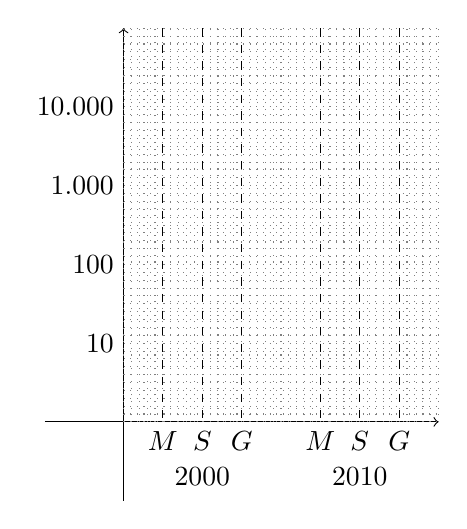
\begin{tikzpicture}[domain=0:5]
\draw[->] (-1,0) -- (4,0);
\draw[->] (0,-1) -- (0,5);
\draw[step=0.1,gray,thin, dotted] (0,0) grid (4,5);
\draw[dashed] (1,5) -- (1,0)node[below] {$S$};
\draw[dashed] (1.5,5) -- (1.5,0)node[below] {$G$};
\draw[dashed] (0.5,5) -- (0.5,0)node[below] {$M$};
\node at (1,-0.7) {$2000$};
\node at (3,-0.7) {$2010$};
\draw[dashed] (3,5) -- (3,0)node[below] {$S$};
\draw[dashed] (3.5,5) -- (3.5,0)node[below] {$G$};
\draw[dashed] (2.5,5) -- (2.5,0)node[below] {$M$};
\node[left] at (0,1) {$10$};
\node[left] at (0,2) {$100$};
\node[left] at (0,3) {$1.000$};
\node[left] at (0,4) {$10.000$};
\end{tikzpicture}
\end{center}
\end{minipage}
\end{center}
No gráfico em escala logarítmica, os valores devem ser marcados na altura dos seus respectivos logaritmos. Utilizando as aproximações $\log 2 \approx 0{,}3$, $\log 5 \approx 0{,}7$ e $\log 11 \approx 1{,}04$, esboce os valores das populações na escala logarítmica à direita:
\begin{enumerate}
\item Qual cidade obteve o maior crescimento?
\item Quais cidades tiveram o maior crescimento em relação aos tamanhos de suas populações?
\end{enumerate}

\ifdefined\prof
\begin{solucao}

	\begin{center}
\begin{tikzpicture}[domain=0:5]
\draw[->] (-1,0) -- (4,0);
\draw[->] (0,-1) -- (0,5);
\draw[step=0.1,gray,thin, dotted] (0,0) grid (4,5);
\draw [fill=session1!80] (0.25,0) rectangle (0.75,4);
\draw [fill=session1!80] (2.25,0) rectangle (2.75,4.04);
\draw [fill=session2!80] (0.75,0) rectangle (1.25,3);
\draw [fill=session2!80] (2.75,0) rectangle (3.25,3.3);
\draw [fill=session4!80] (1.25,0) rectangle (1.75,3.7);
\draw [fill=session4!80] (3.25,0) rectangle (3.75,4);
\draw[dashed] (1,5) -- (1,0)node[below] {$S$};
\draw[dashed] (1.5,5) -- (1.5,0)node[below] {$G$};
\draw[dashed] (0.5,5) -- (0.5,0)node[below] {$M$};
\node at (1,-0.7) {$2000$};
\node at (3,-0.7) {$2010$};
\draw[dashed] (3,5) -- (3,0)node[below] {$S$};
\draw[dashed] (3.5,5) -- (3.5,0)node[below] {$G$};
\draw[dashed] (2.5,5) -- (2.5,0)node[below] {$M$};
\node[left] at (0,1) {$10$};
\node[left] at (0,2) {$100$};
\node[left] at (0,3) {$1.000$};
\node[left] at (0,4) {$10.000$};
\end{tikzpicture}
\end{center}
\begin{enumerate}
\item A cidade com o maior aumento na população  foi Gotham City, com um acréscimo de 5.000 habitantes.
\item As cidades Smallville e Gotham City dobraram suas populações no período, tendo o mesmo crescimento relativo. A população de Metrópolis aumentou apenas 10\%.
\end{enumerate}


\end{solucao}
\fi

\end{document}